\begin{exercise}
    Sei $A := \Bbraces{a_1, a_2}$ und $B := \Bbraces{b_1, b_2, b_3}$ zwei Trägermengen und gemeinsam mit den zyklischen Permutationen $f_A: a_1 \mapsto a_2 \mapsto a_1$ und $f_B: b_1 \mapsto b_2 \mapsto b_3 \mapsto b_1$ zwei Algebren. Zeigen Sie, dass es auf dem direkten Produkt $(C, f_C)$ der beiden keine Unteralgebra gibt, die eine isomorphe Kopie einer der ursprünglichen Algebren ist.
\end{exercise}

\begin{solution}
    Betrachten wir eine beliebige Menge $\emptyset \neq D \subseteq C$, dann gibt es $i \in \{1, 2\} $ und $j \in \{1, 2, 3\}$ so, dass $(a_i, b_j) \in D$ ist. Für alle $k \in \{1, 2\}$ und $l \in \{1, 2, 3\}$ gibt es, wie man im Diagramm erkennen kann, ein $m \in \{0, 1, 2, 3, 4, 5\}$ so, dass $f_C^m(a_i, b_j) = (a_k, b_l)$ und daher ist $(a_k, b_l) \in \langle D \rangle$ also ist $\langle D \rangle = C$. Es sind also die einzigen Unteralgebren von $C$ die trivialen, nämlich $C$ und $\emptyset$, keine von beiden Mengen hat allerdings die gleiche Anzahl von Elementen wie $A$ oder $B$ und daher gibt es auch keine bijektive Abbildung dazwischen also insbesondere keinen Isomorphismus.
    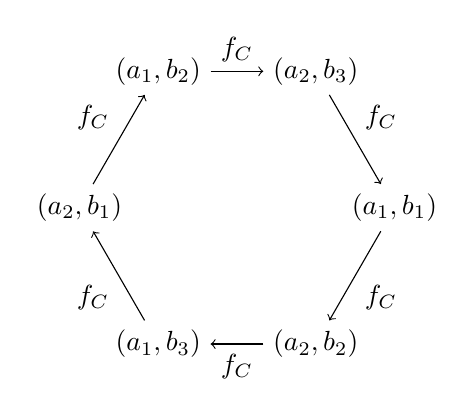
\begin{tikzpicture}[auto]
        \node (1) at (0:2) {$(a_1, b_1)$};
        \node (2) at (300:2) {$(a_2, b_2)$};
        \node (3) at (240:2) {$(a_1, b_3)$};
        \node (4) at (180:2) {$(a_2, b_1)$};
        \node (5) at (120:2) {$(a_1, b_2)$};
        \node (6) at (60:2) {$(a_2, b_3)$};

        \draw[->] (1) to node {$f_C$} (2); 
        \draw[->] (2) to node {$f_C$} (3); 
        \draw[->] (3) to node {$f_C$} (4); 
        \draw[->] (4) to node {$f_C$} (5); 
        \draw[->] (5) to node {$f_C$} (6); 
        \draw[->] (6) to node {$f_C$} (1); 
    \end{tikzpicture}
    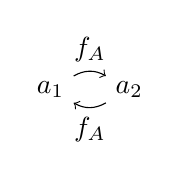
\begin{tikzpicture}[auto, bend left]
        \node (1) at (0,0) {$a_1$};
        \node (2) at (1,0) {$a_2$};

        \draw[->] (1) to node {$f_A$} (2);
        \draw[->] (2) to node {$f_A$} (1);
    \end{tikzpicture}
    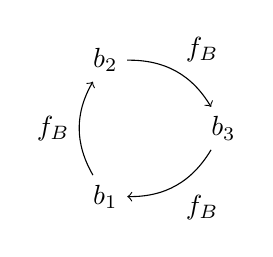
\begin{tikzpicture}[auto, bend left]
        \node (1) at (0:1) {$b_3$};
        \node (2) at (120:1) {$b_2$};
        \node (3) at (240:1) {$b_1$}; 

        \draw[->] (3) to node {$f_B$} (2);
        \draw[->] (2) to node {$f_B$} (1);
        \draw[->] (1) to node {$f_B$} (3);
    \end{tikzpicture}
\end{solution}